\documentclass[oneside]{article}
 \headheight = 25pt
\footskip = 20pt
\usepackage{graphicx}

\usepackage{mdwlist}
\usepackage[T1]{fontenc}
\renewcommand{\rmdefault}{ppl}
\usepackage{fancyhdr}
 \pagestyle{fancy}
 \lhead{\textbf{\textsc{\small Scott O'Connor\\Metaphysics}}}
 \chead{}
 \rhead{\large\textbf{\textsc{Zeno 3}}}
 \lfoot{\footnotesize{\thepage}}
 \cfoot{}
 \rfoot{\footnotesize{\today}}
 \usepackage{longtable,booktabs}
\tolerance=700


\begin{document}
\thispagestyle{fancy}



\section*{Introduction}

Recall again Zeno's overall argument against the existence of motion:

\begin{enumerate}
\item Space is infinitely divisible or not infinitely divisible.
\item  If space is infinitely divisible, motion is impossible.
\item  If space is not infinitely divisible, motion is impossible.
\item  Therefore, motion is impossible (from 1--3).
\end{enumerate}
The conclusion is false; we all do move. Since the conclusion is false, then either the premises do not entail the conclusion or at least one of the premises are false. The argument is valid; the premises do entail the conclusion. So we know at least one of the premises is false. Which one is it? The first premise presents two exhaustive options. There are an infinite number of parts between any two points, or there is not an infinite number of parts between any two points. So the problematic premise must be either the second or third (or both). If we think that one of these premises is false, then we need to find a way of solving the paradoxes that Zeno uses to support them. Doing that will require us to go beyond our ordinary conceptions of motion. You may think you cannot do this, that you cannot conceive motion in any other way than you currently do. But that is what's fascinating about the paradoxes. They push us to rethink motion. They force our minds beyond the limits of what we thought conceivable. 

\section*{The Arrow Paradox}\label{the-arrow-paradox}
The Arrow Paradox primarily supports Premise 3. Zeno asks us to assume that space is finitely divisible. He then proceeds to argue that motion during such  a space is impossible.  There are various presentations of the paradox in antiquity: 
\begin{quote}
The third is \ldots{} that the flying arrow is at rest, which result
follows from the assumption that time is composed of moments \ldots{} .
he says that if everything when it occupies an equal space is at rest,
and if that which is in locomotion is always in a now, the flying arrow
is therefore motionless (Aristotle, \emph{Physics,} 239b30).
\end{quote}

\begin{quote}
Zeno abolishes motion, saying ``What is in motion moves neither in the
place it is nor in one in which it is not'' (Diogenes Laertius, \emph{Lives of
Famous Philosophers,} ix.72).
\end{quote}
\begin{figure}[h]
  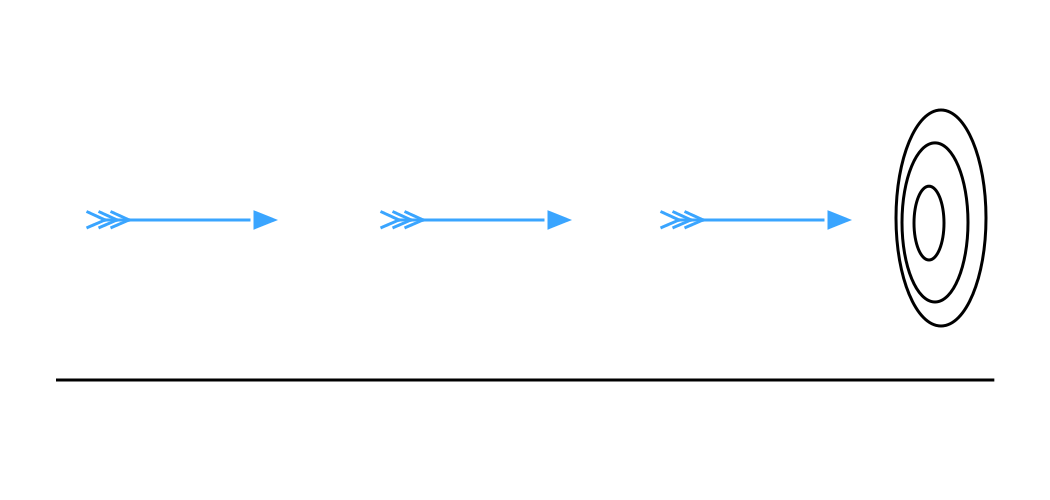
\includegraphics[width=\linewidth]{arrow.png}
\end{figure}
Zeno asks us to consider a moving arrow. The arrow should be in motion at any instant during the time it is moving. What is happening to that arrow at any particular instant? Zeno assumes that it travels no distance during that instant because it occupies a space equal to itself  for the whole instant. 

This is a reasonable assumption. Suppose that the arrow did not occupy a space equal to itself for the whole instant. Perhaps you think it began the instant in one location and ended the instant at a different location. If you think this, then the relevant instant is not really an instant. Recall that we are assuming time is both atomic and that an instant is the smallest measure of time. Thus there cannot be anything shorter than an instant. So what is happening to the arrow at a true instant? It cannot be in motion for all of it because that would require the instant to be divisible into smaller parts.   

Since the entire period of the arrow' motion contains only instants, all of which contain an arrow at rest, Zeno concludes that the the arrow cannot be moving.

\section*{Outline of the Paradox}\label{outline-of-the-paradox}

Assume that space is finitely divisible. Assume also that time is finitely divisible. There are two ways to present the argument:\\

\noindent \textbf{Version 1:}\begin{enumerate}
\item If the arrow moves throughout the period of its flight, then it is moves at each instant of that period. 
\item The arrow occupies a space equal to its own volume at each instant. 
\item If the arrow occupies a space equal to its own volume at an instant, then it is not in motion at that instant. 
\item The arrow is not in motion at any instant of that period (from 2--3).
\item The arrow does not move throughout the period of its flight (from 1 \& 4).\\
\end{enumerate}


\noindent \textbf{Version 2:}

\begin{enumerate}
\item If the arrow moves throughout the period of its flight, then, when it moves, it moves in the present. 
\item The arrow is not in motion in the present. 
\item The arrow does not move throughout the period of its flight (from 1 \& 2). 
\end{enumerate}
Our first version assumes that time is finitely divisible. The second version may not need that assumption. All it requires us to accept that nothing moves during the present. 

 \section*{The Standard Solution}
Motion does exist. To defend its existence, we must either find a solution to the Arrow Paradox, or if we think the Arrow Paradox succeeds, we must solve the paradoxes that Zeno uses to argue against the impossibility of motion in a infinitely divisible space, i.e., we solve the Arrow Paradox or we find a solution to one of the paradoxes Zeno uses to support Premise 2. Here I will discuss the Standard Solution, which charges Zeno with committing the fallacy of composition. This fallacy has the following form: 

\begin{enumerate}
\item[a.] An object, O, has parts, P1, P2, P3 \ldots{Pn}.
\item[b.] None of P1, P2, P3 \ldots{Pn} has propert F. 
\item[c.] O does not have property F...(from a \& b). 
\end{enumerate}
This argument commits a fallacy. Consider a simple example: none of my bodily parts has the property of being 155lb. But that does not entail that I fail to have this property. I am 155lb! Some wholes have the properties of their parts, but some do not. A whole green flag has the properties of its parts, e.g., its parts are green and it is green. But a whole car does not have the properties of all its parts, e.g., the car does not have the property of being an engine, but obviously it has a part that has that property. The Standard Solution to the Arrow Paradox says the following: 
\begin{itemize}
\item An arrow does not move for parts of its flight. 
\item An arrow moves for the whole of its flight. 
\end{itemize}
\begin{figure}[h]
  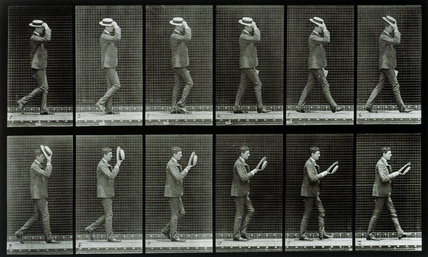
\includegraphics[width=\linewidth]{motion.jpg}
  \caption{At-At Theory of Motion}
\end{figure}
To defend this solution requires that we explain how both these claims could be true. The Standard Solution does this by using  the ``at-at'' theory of motion, which claims that being in motion involves being at different places at different times. All it means for an arrow to move is for it to occupy different locations at different times. The ``at-at'' theory then asks us distinguish between being in motion in or during an instant and   being in motion at an instant. The former is impossible, while the latter is now. Here is a simple summary: 
\begin{enumerate}
\item An object is in motion \textbf{during a period of time} if and only if the object occupies different locations at every instant of that period.
\item An object is in \textbf{motion at an instant} if and only if it occupies different locations immediately before and after that instant. 
\item An objet is \textbf{at rest at an instant} if and only if it is at the same location immediately before and after that instant. 
\end{enumerate}
The at-at theory accepts that the arrow cannot move \textbf{during an instant}, but claims that the arrow can still \textbf{move at an instant}. It does so by occupying different locations before and after that instant. If this is correct, the difference between rest and motion has to do with what is happening at nearby moments and has nothing to do with what is happening during a moment. The arrow counts as moving at an instant because it occupies different locations before and after that instant. The arrow counts as being at rest at an instant because it is not located at different locations before and after that instant.
\newpage
%\subsection{Instantaneous velocity}

\begin{figure}[h]
  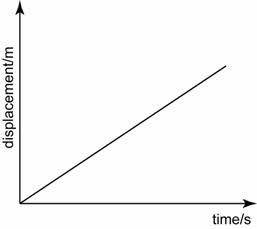
\includegraphics[width=\linewidth]{graph.jpg}
\end{figure}


%- The speed of an object at an instant is the time derivative of the object's position. 

%- This means the object's speed is the limit of its speeds during arbitrarily small intervals of time containing the instant. 

%- The object's speed is the limit of its speed over an interval as the length of the interval tends to zero.

%- The instant must be part of a period in which the arrow is continuously in motion. 

%- The derivative of position x with respect to time t, namely dx/dt, is the arrow's speed, and it has non-zero values at specific places at specific instants during the flight. 



\section*{A Response to the Standard Solution}

The Standard Solution rescues motion by assuming that facts  about an object's location in the future are already fixed: the arrow is moving at an instant because it will be at a different locations in the next instant. This assumes that facts about the arrow's future location determine what is happening to the arrow in the present; it assumes that the future fixes what is happening now. This has caused many to reject the Standard Solution. Surely it is what is happening to the arrow now that determines what happens to it in the future.  

Here is another way to press the worry. Suppose that God exists. Now Suppose he were to wipe the arrow out of existence completely one instant after it has moved. Does the arrow move at the instant before it was annihilated?  

\begin{enumerate}
\item God exists (assume).
\item The arrow occupies location 1, l1, at instant 1, t1.
\item The arrow is moving at t1 if and only if the arrow occupies a different location, l2, at a later instant, t2. 
\item If God destroys the arrow at t2, then the arrow does not occupy l2 at t2.
\item If God destroys the arrow at t2, then the arrow is not moving at t1 (from 1--4).
\item If God does not destroy the arrow at t2, then the arrow does occupy l2 at t2. 
\item If God does not destroy the arrow at t2, then the arrow is moving at t1 (from 1--3, 6)
\item Whether the arrow is moving at t1 depends upon what happens to it in the future (from 5 \& 7) 
\end{enumerate}
\end{document}
